\documentclass{article}
\usepackage[utf8]{inputenc}
\usepackage[T1]{fontenc} % Use modern font encoding that is able to display symbols like < and > easily
\usepackage{parskip} % insert a line between paragraphs instead of indents
\usepackage{geometry} % increase margins, because no-one wants THAT much default margin
\usepackage{hyperref} % make your readers' life easier by including clickable references
\usepackage{enumitem} % customize enumerate, itemize and description
\usepackage{amsthm} % theorems (i.a. proofs)
\usepackage{mathtools} % more beautiful equations
\usepackage{scrextend} % increase i.a. margins
\usepackage{siunitx} % for correct unit displaying
\usepackage{amsmath} % \text{}; split; aligned
\usepackage{listings} % displaying code in listings
\usepackage{caption} % used for subfigures
\usepackage{subcaption} % used for subfigures
\usepackage{algorithm}
\usepackage{algpseudocode}
\usepackage{amssymb} % For example the big-Oh: \mathcal{O}
\usepackage{lscape} % used for landscape tables

% Set the page margin
\geometry{margin=3cm}

% change the visuals of the lstlistings
\definecolor{codegreen}{rgb}{0,0.6,0}
\definecolor{codegray}{rgb}{0.5,0.5,0.5}
\definecolor{codepurple}{rgb}{0.58,0,0.82}
\definecolor{backcolour}{rgb}{0.95,0.95,0.92}
\lstdefinestyle{mystyle}{
    backgroundcolor=\color{backcolour},   
    commentstyle=\color{codegreen},
    keywordstyle=\color{magenta},
    numberstyle=\tiny\color{codegray},
    stringstyle=\color{codepurple},
    basicstyle=\ttfamily\footnotesize,
    breakatwhitespace=false,         
    breaklines=true,                 
    captionpos=b,                    
    keepspaces=true,                 
    numbers=left,                    
    numbersep=5pt,                  
    showspaces=false,                
    showstringspaces=false,
    showtabs=false,                  
    tabsize=4
}
\lstset{style=mystyle}

\hypersetup{
    colorlinks=true,
    urlcolor=blue
}

\title{Web Technology: Memorio \\ 
\large Memory Game Documentation and Assignments (I, II, II)}

\author{
    Group 81:\\
    Menno Hielkema (4591798), Vincent Bockstael (4590694).
}
\date{January 2022}

\begin{document}

\maketitle

\textit{The source code can also be found on github \href{https://github.com/mennohie/memory-project-webdb/}{here}. Furthermore, the game can be played \href{http://memorio-game.herokuapp.com/}{here (https does not work): http://memorio-game.herokuapp.com/}. At last, the brightspace blog post that refers to our project can be found \href{https://brightspace.tudelft.nl/d2l/le/399713/discussions/threads/115930/View?searchText=81}{here}}


\section{Assingment I}

\subsection{HTTP request messages: GET/HEAD}
\subsubsection{The request}

\textbf{Question:} \textit{Write down the HTTP requests you made, the returned responses (e.g. a page has temporarily/permanently moved or is faulty) until you receive the desired contents with status code 200 OK. Always use HEAD first to retrieve meta-­data about the resource.}

using \texttt{telnet reddit.com 80} we start the connection with \textit{reddit.com}. Next, we make a \texttt{HEAD} request to \texttt{/r/tudelft}. This is done with the following HTTP request:

\begin{lstlisting}[]
HEAD /r/tudelft HTTP/1.1
host:www.reddit.com
\end{lstlisting}

From this we get the following response


\begin{lstlisting}[]
HEAD /r/tudelft HTTP/1.1
host:www.reddit.com

HTTP/1.1 301 Moved Permanently
Retry-After: 0
Location: https://www.reddit.com/r/tudelft
Content-Length: 0
Accept-Ranges: bytes
 ...
\end{lstlisting}

This indicates that it moved the request to a new location: \texttt{https://www.reddit.com/r/tudelft}. From this we say that it moved the HTTP request to a https request. This means we will require \textbf{openssl} to connect to \texttt{reddit.com}. We do this with the following:

\begin{lstlisting}
openssl s_client -crlf -connect www.reddit.com:443
\end{lstlisting}

Then making the same \texttt{HEAD} request we made earlier gives us the following:

\begin{lstlisting}
HEAD /r/tudelft HTTP/1.1
host:www.reddit.com

HTTP/1.1 200 OK
Connection: keep-alive
Cache-control: private, s-maxage=0, max-age=0, must-revalidate, no-store
Content-Type: text/html; charset=utf-8
\end{lstlisting}

The status \texttt{200 OK} indicates that the request was successful. Now we will make the \texttt{GET} request.

\begin{lstlisting}
GET /r/tudelft HTTP/1.1
host:www.reddit.com

HTTP/1.1 200 OK
Connection: keep-alive
Cache-control: private, s-maxage=0, max-age=0, must-revalidate, no-store
Content-Type: text/html; charset=utf-8
\end{lstlisting}

\subsubsection{The response}
\textbf{Question}: \textit{Does the content you received correspond to what you see when accessing the resource with your browser?}

The content appears to be html text that is effectively (and unreadably) compressed in the response body. When loading the html text in a browser the result appears to look like the a reddit page.

\subsubsection {}
\textbf{Question}: \textit{Open your browser’s developer tools and head to https://www.reddit.com/r/TUDelft/. Take a look at the response header of the first resource retrieved with status code 200 OK: what does its Cache-Control header field mean?}

The \texttt{Cache-control} says \texttt{private, s-maxage=0, max-age=0, must-revalidate, no-store}

As quoted from the documentation \href{https://developer.mozilla.org/en-US/docs/Web/HTTP/Headers/Cache-Control}{here}:

\begin{itemize}
    \item The \texttt{max-age=0} response directive indicates that the response remains fresh until 0 seconds after the response is generated.
    \item The \texttt{s-maxage} response directive also indicates how long the response is fresh for (similar to \texttt{max-age}) — but it is specific to shared caches, and they will ignore max-age when it is present.
    \item The \texttt{must-revalidate} response directive indicates that the response can be stored in caches and can be reused while fresh. Once it becomes stale, it must be validated with the origin server before reuse.
    \item The \texttt{private} response directive indicates that the response can be stored only in a private cache (e.g. local caches in browsers).
    \item The \texttt{no-store} response directive indicates that any caches of any kind (private or shared) should not store this response.
\end{itemize}


So, since the \texttt{max-age} and \texttt{s-max-age} are set to 0, the response is not-fresh immediately after its recipient got the response. In combination with \texttt{must-revalidate} this requires the page to refresh from the origin server before reuse instead of using any stored caches. However, generally, the response should not be stored at all (by \texttt{no-store}). 

This seems as a logical choice for reddit, as the page should be refreshed with its content on usage to contain the latest news.

\subsubsection{}
\textbf{Question} \textit{If we stick to the resource considered in 1.3), what do we learn about the type of encodings your browser supports?}

The value for the \texttt{Content-encoding} is \texttt{gzip}. This suggests that the browser used (Google Chrome) supports gzip. 

\subsection{HTTP request messages: PUT}

We make a \texttt{PUT} request to \texttt{httpbin.org/put} with "Hello World!" and obtain a response as follows:


\begin{lstlisting}
PUT /put HTTP/1.1
host:httpbin.org
Content-type:text/plain
Content-length:12

Hello World!
HTTP/1.1 200 OK
Date: Sat, 15 Jan 2022 19:46:10 GMT
Content-Type: application/json
Content-Length: 338
Connection: keep-alive
Server: gunicorn/19.9.0
Access-Control-Allow-Origin: *
Access-Control-Allow-Credentials: true

{
  "args": {},
  "data": "Hello World!",
  "files": {},
  "form": {},
  "headers": {
    "Content-Length": "12",
    "Content-Type": "text/plain",
    "Host": "httpbin.org",
    "X-Amzn-Trace-Id": "Root=1-61e3247e-139fbc4c79072b7211a6c33b"
  },
  "json": null,
  "origin": "85.144.203.142",
  "url": "http://httpbin.org/put"
}

\end{lstlisting}

\subsubsection{Other resource}

\textbf{Question}: \textit{What happens if you try to replace /put in this exercise with another resource (e.g. /myfile)? Does the httpbin.org server allow the creation of a new resource?}

If we make a \texttt{PUT} request to \texttt{httpbin.org/myfile}, the \texttt{httpbin.org} server denies the request as it can not find \texttt{/myfile} (it gives a 404 Not Found error code).

\begin{lstlisting}
PUT /myfile HTTP/1.1
host:httpbin.org
Content-type:text/plain
Content-length:12

HTTP/1.1 404 NOT FOUND
Date: Sat, 15 Jan 2022 19:48:21 GMT
Content-Type: text/html
Content-Length: 233
Connection: keep-alive
Server: gunicorn/19.9.0
Access-Control-Allow-Origin: *
Access-Control-Allow-Credentials: true

<!DOCTYPE HTML PUBLIC "-//W3C//DTD HTML 3.2 Final//EN">
<title>404 Not Found</title>
<h1>Not Found</h1>
<p>The requested URL was not found on the server.  If you entered the URL manually please check your spelling and try again.</p>
Connection closed by foreign host.
\end{lstlisting}

\subsubsection{Content-length}

\textbf{Question}: \textit{The Content-­length is exactly the number of characters (12 - we count the whitespace as well!) of Hello World!. What happens if the Content-length field is smaller or larger than the exact number of characters in the content?}

If the content-length is longer than the actual content, the request is still process and the server responds with status OK (200)
If the Content-length is too short (shorter than the length of the content), The server responds with a Bad Request (400).

\subsection{Basic authentication}

\subsubsection{}
\textbf{Question}: \textit{First, open \href{http://httpbin.org/basic-auth/user/passwd}{http://httpbin.org/basic-auth/user/passwd} in your browser. You should see a dialogue, requesting username and password. Use user as username and passwd as password (it is just a coincidence that the actual username and password is the same as the URL path). Reload the web page—do you have to fill in the login details again? Why or why not?}

The resulting page shows the following message:

\begin{texttt}
{\\
  "authenticated": true, \\
  "user": "user"\\
}\\
\end{texttt}


When the page is reloaded the credentials are not asked again. This is because the \texttt{Authorization} header has been set in the cookies of the browser. The \texttt{Authorization} header looks as follows:

\begin{texttt}
{\\
Authorization: Basic dXNlcjpwYXNzd2Q=
}\\
\end{texttt}

Apperantly, the \texttt{Authorization} header correctly authorizes the access to the page. If the header is removed from cookies, the credentials are asked again.

\subsubsection{}

If we make the same request with \texttt{telnet}, we get the following response:

\begin{lstlisting}
HEAD /basic-auth/user/passwd HTTP/1.1
host:httpbin.org

HTTP/1.1 401 UNAUTHORIZED
Date: Sun, 16 Jan 2022 16:31:28 GMT
Content-Length: 0
Connection: keep-alive
Server: gunicorn/19.9.0
WWW-Authenticate: Basic realm="Fake Realm"
Access-Control-Allow-Origin: *
Access-Control-Allow-Credentials: true
\end{lstlisting}

We get an unauthorized status response. If we add a (correct) \texttt{Authorization} header to the request, we actually are able to make the request. We get a correct \texttt{Authorization} header by encoding our username and password. Or, we can copy the cookie value from the browser.

\begin{lstlisting}
HEAD /basic-auth/user/passwd HTTP/1.1
host:httpbin.org
Authorization: Basic dXNlcjpwYXNzd2Q=

HTTP/1.1 200 OK
Date: Sun, 16 Jan 2022 16:34:16 GMT
Content-Type: application/json
Content-Length: 47
Connection: keep-alive
Server: gunicorn/19.9.0
Access-Control-Allow-Origin: *
Access-Control-Allow-Credentials: true
\end{lstlisting}

Now, if we retry this without the \texttt{Authorization} header, analogous to reloading the page, we again get an unauthorized response. While the browser stores the \texttt{Authorization} header, \texttt{telnet} does not.

\begin{lstlisting}
HEAD /basic-auth/user/passwd HTTP/1.1
host:httpbin.org

HTTP/1.1 401 UNAUTHORIZED
Date: Sun, 16 Jan 2022 16:36:52 GMT
Content-Length: 0
Connection: keep-alive
Server: gunicorn/19.9.0
WWW-Authenticate: Basic realm="Fake Realm"
Access-Control-Allow-Origin: *
Access-Control-Allow-Credentials: true
\end{lstlisting}


\subsection{Web programming project: board game app}

\subsubsection{Memory}
\textbf{Question}: \textit{First of all, settle on the game you will implement in your team.}

We chose to make a memory game. To be specific a memory game with a timer.

\subsubsection{Example Games}
\textbf{Question}: \textit{Find three examples of your chosen board game (in 2D) that can be played online in a modern browser (laptop or desktop, not a mobile device). Consider the web application’s design (focus on the game screen) based on the web design principles covered in class: to what extent do they fulfill them? Record the game URLs.}

\href{pairs.one}{\textbf{Pairs.one}}
\begin{itemize}
    \item can be played in multiple ways (Local, solo, 2 player, random )
    \item A custom board size can be made (from 4x4 to 8x8)
    \item A custom amount of players can be set (1 to 4)
    \item Animations are smooth
    \item Style is concise, but a bit boring
    \item There is no sound
    \item With a small amount of clicks a game can be started
\end{itemize}


\href{playingcards.io}{\textbf{Playingcards.io}}
\begin{itemize}
    \item has a memory game with the 52 playing cards.
    \item The cards can be used to play memory up to 4 cards.
    \item A custom point counter is used
Cards have to be dragged to the users deck if the cards match.
    \item There is a lot of freedom, but a bit too much.
It is not very evident how to play a “matching” game with this.
    \item The design is not distractive.
\end{itemize}


\href{https://matchthememory.com/}{\textbf{Match the Memory}}
\begin{itemize}
    \item Custom board choices, and a couple different saved board choices
    \item Simple design
    \item You have to scroll for bigger games which is not really great
    \item Simple sounds
    \item Customizable amount of pairs
    \item Only single player
\end{itemize}

\subsubsection{Positives and Negatives}
\textbf{Question}: \textit{Which game features in the game examples of 4.2) stand out positively and which stand out negatively (e.g. particular animations, sounds, information conveyed about the game to the players …)? Why? Discuss three positive and three negative features.}

\textbf{Positives}
\begin{itemize}
    \item Customizability (in all three)
    \item Smooth animation (in Pairs.io)
    \item No distractions (in Playingcards.io and Pairs.io)
    \item Few required clicks to start a game (in Playingcards.io and Pairs.io)
\end{itemize}

\textbf{Negatives}
\begin{itemize}
    \item Too much freedom (in Playingcards.io)
    \item Hard to start a game (in Match the Memory)
    \item Non-self explanatory design (in Playingcards.io)
\end{itemize}

\subsection{Design your own board game app}

\subsubsection{Splash Screen}
\textbf{Question}: \textit{Create a design for the splash screen (also known as entry page): think of a name for your application, a short description & a logo. Feel free to use media (images, sound) with a Creative Commons license. The noun project can be a useful resource for game pieces.}

The design of our splash screen can be found in figure \ref{fig:splash_screen}

\begin{figure}[t]
    \centering
    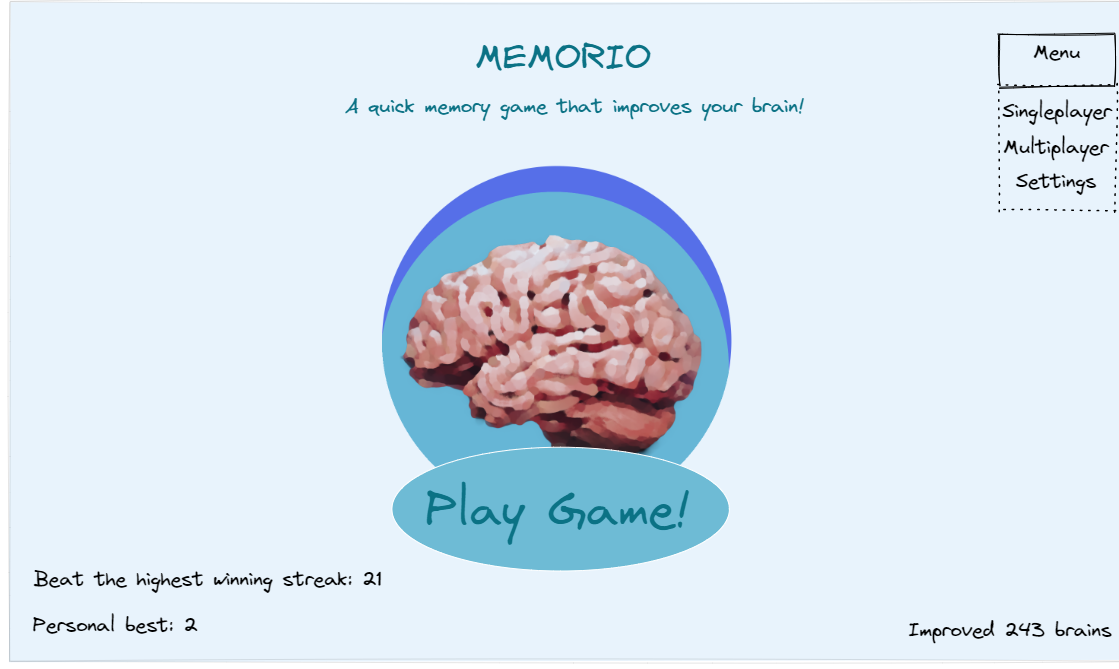
\includegraphics[width=\textwidth]{splash.png}
    \caption{The design of our splash Screen}
    \label{fig:splash_screen}
\end{figure}

\subsubsection{Game Screen}

\textbf{Question}: \textit{Create a design for the game screen, keeping the requirements listed above in mind as well as your findings in Exercise 4.3). You have a lot of artistic freedom in designing the board and game information.}

The design of our game screen can be found in figure \ref{fig:game_screen}


\begin{figure}[t]
    \centering
    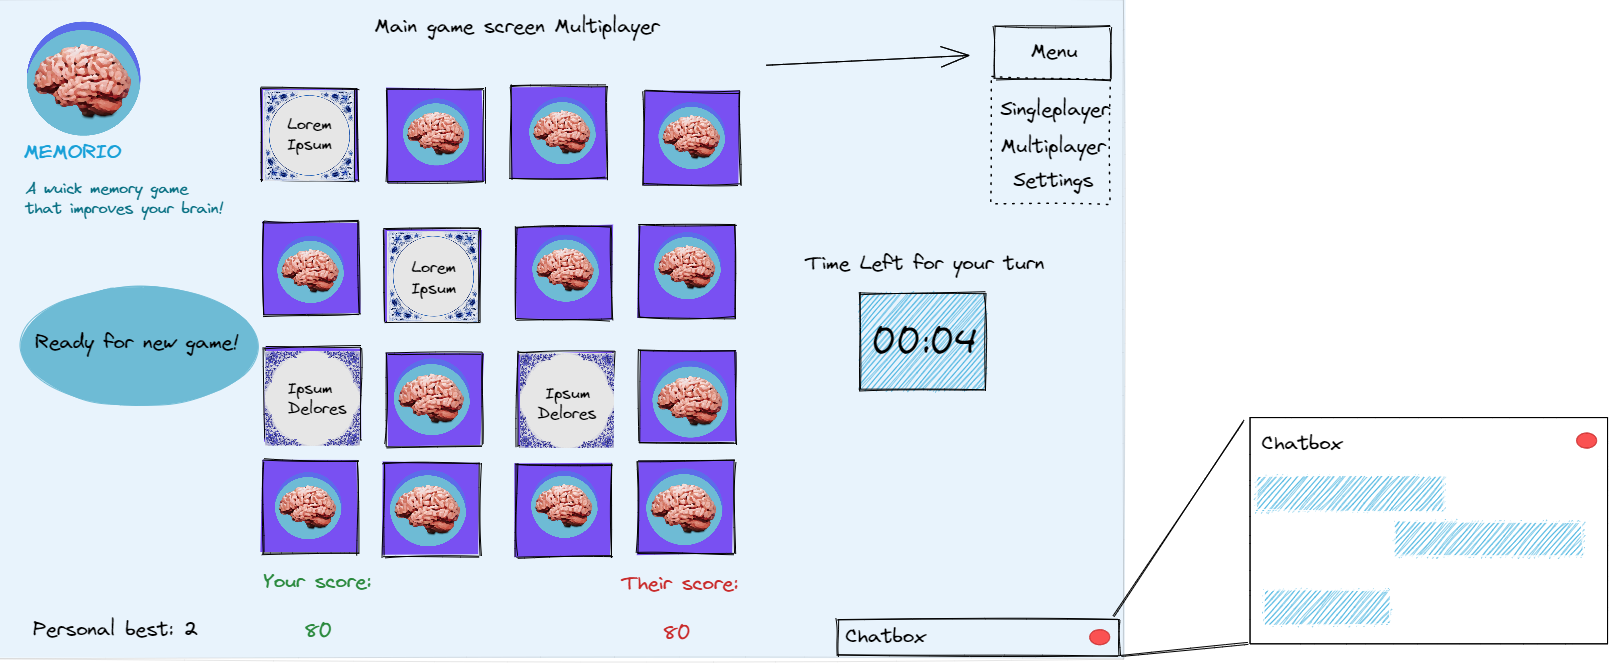
\includegraphics[width=1.0\textwidth]{game.png}
    \caption{The design of our game screen}
    \label{fig:game_screen}
\end{figure}

\subsubsection{Blog Post}
\textbf{Memorio} - a quick memory game that improves your brain - that is our motto.

The game is a fast-paced two-player memory game with a time limit of (to be determined) seconds per turn. he images on the memory cards show "Delfts Blauwe" tiles with arbitrary wisdom proverbs The game improves your brain in two ways:

\begin{itemize}
    \item It increases your short term memory by playing the memory card game
    \item It increases your wisdom by reading the wisdom proverbs. ;-)
\end{itemize}

Furthermore, we chose to show statistics on how many brains were improved (amount of games played). We also show the highest winning streak on the splash screen together with your own personal best winning streak.

\subsubsection{Initial \texttt{game.html} and \texttt{splash.html}}

The initial game screen html file and splash screen html file can be seen \href{https://github.com/mennohie/memory-project-webdb/blob/d7e7d1c3f0c67e9dbcf54ca13b5a8b2b9df77845/public/game.html}{here} and \href{https://github.com/mennohie/memory-project-webdb/blob/d7e7d1c3f0c67e9dbcf54ca13b5a8b2b9df77845/public/splash.html}{here} respectively.

\pagebreak

\section{Assignment II}

\subsection{Boilerplate Code}


The result from creating the boilerplate code with the express can be found \href{https://github.com/mennohie/memory-project-webdb/commit/0c1ac83a4d52c7b3378ce29ae22cf216194b26d4}{here} 

\subsection{Client-side Javascript}

\subsubsection{Components and Functionalities}
\textbf{Question}: \textit{Before you start coding, you need to have a plan of what needs to be done. Focus on your game.html page. We will deal with splash.html in the next assignment. Check the required functionalities of your game listed in the first web assignment once again. Make a list of all interactive UI elements you need and their functionality.}

In figure \ref{fig:uml_components} an overview of all the components (not strictly UML, despite the look) and functionalities of the game can be found. 

\begin{figure}[t]
    \centering
    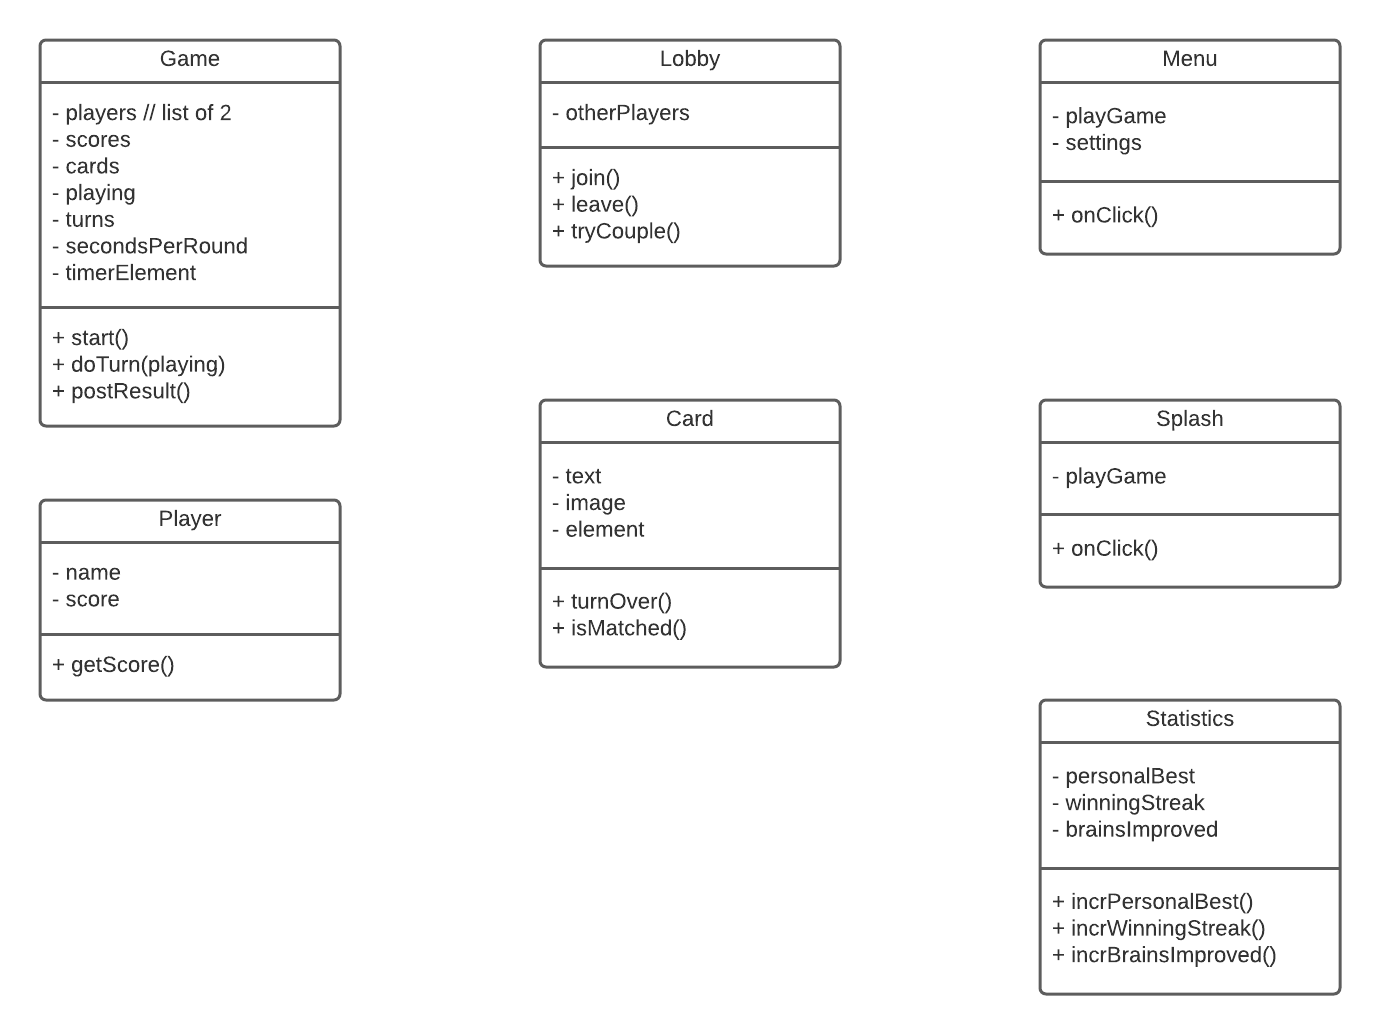
\includegraphics[height=0.5\textheight]{uml-memorio.png}
    \caption{An overview of the game components and their functionalities}
    \label{fig:uml_components}
\end{figure}

\subsubsection{Design Patterns}

\textbf{Question}: \textit{Think about the design of your JavaScript code—which aspects of your action plan can you translate into objects? It will make sense to separate the game logic from the game interface. For example, you might want to create different objects for: the game state; the game board; the game items. Choose at least one of the object design patterns introduced in the lecture and implement your objects accordingly. The basic constructor pattern is the simplest one to implement, the module pattern is more complex but preferable for code maintainability. Feel free to try more than one design pattern. This is your chance to use and learn about the introduced design patterns in more detail!}

We use a \textit{Class} \href{https://developer.mozilla.org/en-US/docs/Web/JavaScript/Reference/Classes}{ES2015} to design several client-side objects such as: 

\begin{itemize}
    \item \href{https://github.com/mennohie/memory-project-webdb/blob/34a6ba670b041a60b2915c33ae894a1768a40f82/memorio/public/javascripts/game.js}{Game}
    \item \href{https://github.com/mennohie/memory-project-webdb/blob/34a6ba670b041a60b2915c33ae894a1768a40f82/memorio/public/javascripts/cardGrid.js}{cardGrid}
\end{itemize}

We also use the \textit{Constructor} design pattern for client-side \href{https://github.com/mennohie/memory-project-webdb/blob/34a6ba670b041a60b2915c33ae894a1768a40f82/memorio/public/javascripts/cardGrid.js}{Card}

At last, we use a \textit{prototype} design pattern for server-side \href{https://github.com/mennohie/memory-project-webdb/blob/34a6ba670b041a60b2915c33ae894a1768a40f82/memorio/game.js}{Game}

\subsubsection{Client Side Memory Game}

We implemented a basic client side (non-functional) game \href{https://github.com/mennohie/memory-project-webdb/commit/6b39c67993f45905e8d1d087a9392466e1f71779}{here}. The basic game object classes exist and basic interactions work.

\subsection{Node.js}

The bulk of the implementing work was done here. The final result apart from some styling with css is what has been done for this part.

\pagebreak
\section{Assignment III}

\subsection{CSS}

\subsubsection{Splash Screen}

\textbf{Question}: \textit{First, work on your splash screen and style the page with CSS according to your design. To ensure that everyone learns the basics of CSS, we provide a list of must-have CSS properties. Your code must include at least one instance of each of the following: pseudo-classes :hover and :active; pseudo-elements ::after and ::before; display:grid and position:absolute; a CSS animation.}

\textbf{pseudo-classes}:
We add a \textit{hover} effect on the large play button. It increases in size. Furthermore, we add an \textit{active} effect on the button that changes the color of the image. At last, we add a transition property to the hover effect such that the transitions are smooth.

\begin{lstlisting}
.play-image:hover {
  transform: translate(-50%, -50%) scale(1.1);
  transition-duration: 0.5s;
}

.play-image:active {
  filter: hue-rotate(180deg);
}
\end{lstlisting}

\textbf{pseudo-elements}

We add a fire emoticon before and after the statistics displayed on the splash screen. We also add a "\texttt{\#}" symbol before the statistic value.

\begin{lstlisting}
.stat-value::before {
  content: "#";
}

.stat::before {
  font-weight: normal;
  content: "\01F525";
  animation: stat-enter 3.0s
}

.stat::after {
  font-weight: normal;
  content: "\01F525";
  animation: stat-enter 4.0s
}
\end{lstlisting}

\textbf{Grid and Absolute Position} 

We use a grid display to divide the splash screen into areas with content. The same grid template is used for the splash screen as the game screen. This gives it a coherent layout.

We use an absolute postion to center the image in a grid cell.
\begin{lstlisting}
.play-image {
  position: absolute;
  top: 50%;
  left: 50%;
  height: 100%;
  transform: translate(-50%, -50%);
  transition-duration: 0.5s;
  animation: image-enter 1s 1;
}
\end{lstlisting}

\textbf{CSS Animation}

At last, we use an animation when the page is loaded. The large image is scaled in \textbf{y} direction, i.e. it starts flat and than stretches out to the original image. Also the opacity of the statistics starts at \textbf{0} and transforms to \textbf{1}.

\begin{lstlisting}
@keyframes image-enter {
	0% {
		transform: translate(-50%, -50%) scale(0, .025);
	}
	50% {
		transform: translate(-50%, -50%) scale(1, .025);
	}
}
\end{lstlisting}

\subsubsection{Game Screen CSS}



\textbf{Question}: \textit{Next, tackle the CSS for your game screen. The look of the game screen should be coherent with the splash screen. The two are likely to share basic CSS settings (colors, fonts, etc.); try to be efficient and do not duplicate existing CSS code.}

The game screen shares a lot of elements with the splash screen. An important difference is that the game board is in the center instead of the play button. The game board has a \texttt{card-grid-container} that has a grid layout. The container contains all cards, and has a 4 by 4 layout achieved as follows:

\begin{lstlisting}
.card-grid-container {
  display: grid;
  justify-content: center;
  grid-template-columns: auto auto auto auto;
  grid-gap: 5px;
  padding: 5px;
}
\end{lstlisting}

\subsection{Media Query}

\textbf{Question}: \textit{To ensure that your players are aware of the screen size limitations (i.e. the game works well on a larger screen), use media queries to alert players if their screen resolution is below a sufficiently large minimum. How exactly the alert looks like is up to you. What exactly the screen resolution minimum is, is up to you. There is no need to actually try your app on different physical devices, Firefox (other major browsers have similar tooling) has a Responsive Design Mode tool that provides good simulations of various devices.}

We developed the game for regular wide screen devices, so any device with smaller screens than roughly \textit{1100px} width will probably not have a pleasant experience. To prevent this, we set the display of the entire main section to none. Instead we show an error message:

\begin{lstlisting}[language=html]
<div class="alert-not-available">
  We are sorry, it appears you have tunnel vision. Widen your view to a width of 1100px
</div>
\end{lstlisting}

\begin{lstlisting}
@media only screen and (max-width: 1100px) {
  .main-grid {
    display: none;
  }

  .alert-not-available {
    display: block;
  }
}
\end{lstlisting}

\subsection{Templating}

The following html was written on the splash page. (splash.html)
\begin{lstlisting}
  <p class="scores">Beat the highest winning score: <span id="top-score"></span></p>
  <p class="scores">Personal best: <span id="personal-best"></span></p>
  <p class="scores">Improved <span id="brains-improved"></span> brains</p>
\end{lstlisting}

A client can obtain relevant server info by going to the endpoint "/publicserverdata". A user does not know that, but instructions are given in the onLoad.js file.

server-side app.js
\begin{lstlisting}
// @ts-ignore
app.get('/publicserverdata', function (req, res) {
  res.send(gameStatus)
})
\end{lstlisting}

client-side onLoad.js
\begin{lstlisting}
/* eslint-disable no-undef */
if (getCookie('highScore') === undefined) {
  // Cookie is stored for 5 years
  setCookie('highScore', 0, 1825)
}

serverInfo = JSON.parse(getResponse(window.location.protocol + '//' + window.location.host + '/publicserverdata'))

document.getElementById('personal-best').innerHTML = getCookie('highScore')
document.getElementById('brains-improved').innerHTML = serverInfo.gamesCompleted
document.getElementById('top-score').innerHTML = serverInfo.highScore
\end{lstlisting}

As you can see, onLoad.js injects serverdata in the shown spans of splash.html. Using AJAX instead of js would probably make it possible to update serverdata real-time instead of every refresh.

A personal best is not stored on the server but in the cookies of a browser. It is a more simple solution than server-side personal data storage, which would probably require registration and login.

Unfortunately, using ejs files did not properly work for some reason. However, this method seems to work fine too.

\end{document}


